\chapter{Batch Python Scripting}
\label{chap:BatchPythonScripting}

Python scripting can be leveraged in two ways within ParaView.  First,
Python scripts can automate the setup and execution of visualizations by
performing the same actions as a user at the GUI.  Second, Python scripts
can be run inside pipeline objects, thereby performing parallel
visualization algorithms.  This chapter describes the first mode, batch
scripting for automating the visualization.

Batch scripting is a good way to automate mundane or repetitive tasks, but
it is also a critical component when using ParaView in situations where the
GUI is undesired or unavailable.  The automation of Python scripts allows
you to leverage ParaView as a scalable parallel post-processing framework.
We are also leveraging Python scripting to establish \emph{in-situ}
computation within simulation code (a.k.a. co-processing).

This tutorial gives only a brief introduction to Python scripting.  The
most recent and complete documentation is kept on the ParaView Wiki.

\begin{quote}
  \href{http://www.paraview.org/Wiki/ParaView/Python_Scripting}{http://www.paraview.org/Wiki/ParaView/Python\_Scripting}
\end{quote}

\section{Starting the Python Interpreter}
\label{sec:StartingThePythonInterpreter}

There are many ways to invoke the Python interpreter.  The method you use
depends on how you are using the scripting.  The easiest way to get a
python interpreter, and the method we use in this tutorial is to select
\gui{Tools} \ra \gui{Python Shell} from the menu.  This will bring up a
dialog box containing most principally a text area where you can interact
with the Python interpreter.

\begin{inlinefig}
  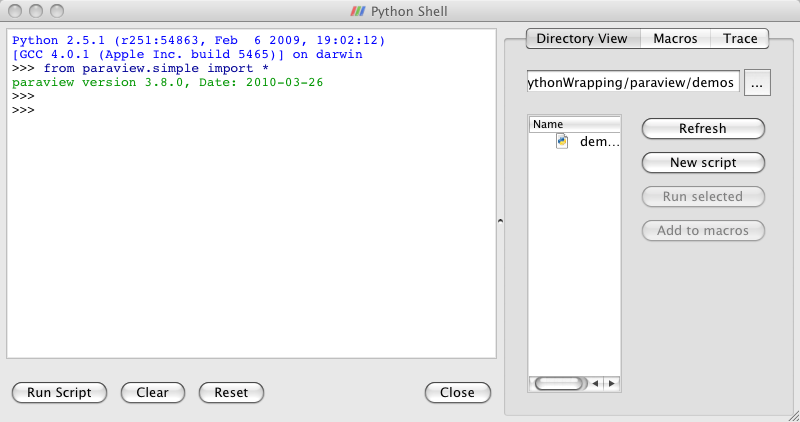
\includegraphics[width=2.5in]{images/PythonShellDialog}
\end{inlinefig}

If you are right now most interested in getting started on writing scripts,
feel free to skip to the next section past the discussion of the other ways
to invoke scripting.

ParaView comes with two command line programs that execute Python scripts:
\commandline{pvpython} and \commandline{pvbatch}.  They are similar to the
\commandline{python} executable that comes with Python distributions in
that they accept Python scripts either from the command line or from a file
and they feed the scripts to the Python interpreter.

The difference between \commandline{pvpython} and \commandline{pvbatch} is
subtle and has to do with the way they establish the visualization
service.  \commandline{pvpython} is roughly equivalent to the
\commandline{paraview} client GUI with the GUI replaced with the Python
interpreter.  It is a serial application that connects to a ParaView server
(which can be either builtin or remote).  \commandline{pvbatch} is roughly
equivalent to \commandline{pvserver} except that commands are taken from a
Python script rather than from a socket connection to a client.  It is a
parallel application that can be launch with \commandline{mpirun} (assuming
it was compiled with MPI), but it cannot connect to another server; it is
its own server.  In general, you should use \commandline{pvpython} if you
will be using the interpreter interactively and \commandline{pvbatch} if
you are running in parallel.

It is also possible to use the ParaView Python modules from programs
outside of ParaView.  This can be done by pointing the \texttt{PYTHONPATH}
environment variable to the location of the ParaView libraries and Python
modules and pointing the \texttt{LD\_LIBRARY\_PATH} (on Unix/Linux/Mac) or
\texttt{PATH} (on Windows) environment variable to the ParaView libraries.
Running the Python script this way allows you to take advantage of
third-party applications such as IDLE.  For more information on setting up
your environment, consult the ParaView Wiki.

\section{Creating a Pipeline}
\label{sec:CreatingAPipeline}

The first thing any ParaView Python script must do is load the
\textpy{paraview.simple} module.  This is done by invoking
\begin{python}
from paraview.simple import *
\end{python}
In general, this command needs to be invoked at the beginning of any
ParaView batch Python script.  This command is automatically invoked for
you when you bring up the scripting dialog in ParaView, but you must add it
yourself when using the Python interpreter in other programs (including
\commandline{pvpython} and \commandline{pvbatch}).

The \textpy{paraview.simple} module defines a function for every source,
reader, filter, and writer defined in ParaView.  The function will be the
same name as shown in the GUI menus with spaces and special characters
removed.  For example, the \pyfunc{Sphere} function corresponds to
\gui{Sources} \ra \gui{Sphere} in the GUI and the \pyfunc{PlotOverLine}
function corresponds to \gui{Filters} \ra \gui{Data Analysis} \ra \gui{Plot
  Over Line}.  Each function creates a pipeline object, which will show up
in the pipeline browser (with the exception of writers), and returns an
object that is a proxy that can be used to query and manipulate the
parameters of that pipeline object.

There are also several other functions in the \textpy{paraview.simple}
module that perform other manipulations.  For example, the pair of
functions \pyfunc{Show} and \pyfunc{Hide} turn on and off, respectively,
the visibility of a pipeline object in a view.  The \pyfunc{Render}
function causes a view to be redrawn.

\begin{exercise}{Creating and Showing a Source}
  \label{ex:CreatingAndShowingASource}%
  If you have not already done so, open the Python shell in the ParaView
  GUI by selecting \gui{Tools} \ra \gui{Python Shell} from the menu.  You
  will notice that
  \begin{python}
from paraview.simple import *
  \end{python}
  has been added for you.

  Create and show a \gui{Sphere} source by typing the following in the
  Python shell.
  \begin{python}
sphere = Sphere()
Show()
Render()
  \end{python}

  The \pyfunc{Sphere} command creates a sphere pipeline object.  Once it is
  executed you will see an item in the pipeline browser created.  We save a
  handle to the pipeline object in the variable \textpy{sphere}.  We are
  not using this variable (yet), but it is good practice to save references
  to your pipeline objects.

  The following \pyfunc{Show} command turns on visibility of this object in
  the view, and the subsequent \pyfunc{Render} causes the results to be
  seen.  At this point you can interact directly with the GUI again.  Try
  changing the camera angle in the view with the mouse.
\end{exercise}

\begin{exercise}{Creating and Showing a Filter}
  \label{ex:CreatingAndShowingAFilter}%
  Creating filters is almost identical to creating sources.  By default,
  the last created pipeline object will be set as the input to the newly
  created filter, much like when creating filters in the GUI.

  This exercise is a continuation of
  Exercise~\ref{ex:CreatingAndShowingASource}.  You will need to finish
  that exercise before beginning this one.

  Type in the following script in the Python shell that hides the sphere
  and then adds the shrink filter to the sphere and shows that.

  \pyfuncindex{Hide}\pyfuncindex{Show}\pyfuncindex{Shrink}\pyfuncindex{Render}
  \begin{python}
Hide()
shrink = Shrink()
Show()
Render()
  \end{python}

  The sphere should be replaced with the output of the \pyfunc{Shrink}
  filter, which makes all of the polygons smaller to give the mesh an
  exploded type of appearance.
\end{exercise}

So far as we have built pipelines we have accepted the default parameters
for the pipeline objects.  As we have seen in the exercises of
Chapter~\ref{chap:BasicUsage}, it is common to have to modify the
parameters of the objects using the object inspector.

In Python scripting, we use the handle returned from the creation functions
to manipulate the pipeline objects.  These handles are in fact Python
objects with class attributes that correspond to the same properties you
set in the Object Inspector.  They have the same names as those in the
object inspector with spaces and other illegal characters removed.  You can
set them by simply assigning them a value.

\begin{exercise}{Changing Pipeline Object Parameters}
  \label{ex:ChangingPipelineObjectParameters}%
  This exercise is a continuation of Exercises
  \ref{ex:CreatingAndShowingASource} and
  \ref{ex:CreatingAndShowingAFilter}.  You will need to finish those
  exercises before beginning this one.

  Recall that we have so far created two Python variables, \textpy{sphere}
  and \textpy{shrink}, that are handles to the corresponding pipeline
  objects.  First, enter the following command into the Python shell to get
  the current value of the \gui{Theta Resolution} parameter of the sphere.

  \begin{python}
print sphere.ThetaResolution
  \end{python}

  The Python interpreter should respond with the result \textpy{8}.  (Note
  that using the \textpy{print} keyword, which instructs Python to output
  the arguments to standard out, is superfluous here as the Python shell
  will output the result of any command anyway.)  Let us double the number
  of polygons around the equator of the sphere by changing this parameter.

  \begin{python}
sphere.ThetaResolution = 16
Render()
  \end{python}

  The shrink filter has only one parameter, \gui{Shrink Factor}.  We can
  adjust this factor to make the size of the polygons larger or smaller.
  Let us change the factor to make the polygons smaller.

  \begin{python}
shrink.ShrinkFactor = 0.25
Render()
  \end{python}

  You may have noticed that as you type in Python commands to change the
  pipeline object parameters, the GUI in the object inspector updates
  accordingly.
\end{exercise}

So far we have created only non-branching pipelines.  This is a simple and
common case and, like many other things in the \textpy{paraview.simple}
module, is designed to minimize the amount of work for the simple and
common case but also provide a clear path to the more complicated cases.
As we have built the non-branching pipeline, ParaView has automatically
connected the filter input to the previously created object so that the
script reads like the sequence of operations it is.  However, if the
pipeline has branching, we need to be more specific about the filter
inputs.

\begin{exercise}{Branching Pipelines}
  \label{ex:BranchingPipelines}%
  This exercise is a continuation of Exercises
  \ref{ex:CreatingAndShowingASource} through
  \ref{ex:ChangingPipelineObjectParameters}.  You will need to finish
  Exercises \ref{ex:CreatingAndShowingASource} and
  \ref{ex:CreatingAndShowingAFilter} before beginning this one
  (Exercise~\ref{ex:ChangingPipelineObjectParameters} is optional).

  Recall that we have so far created two Python variables, \textpy{sphere}
  and \textpy{shrink}, that are handles to the corresponding pipeline
  objects.  We will now add a second filter to the sphere source that will
  extract the wireframe from it.  Enter the following in the Python shell.

  \pyfuncindex{ExtractEdges}
  \begin{python}
wireframe = ExtractEdges(Input=sphere)
Show()
Render()
  \end{python}

  An \gui{Extract Edges} filter is added to the sphere source.  You should
  now see both the wireframe of the original sphere and the shrunken
  polygons.

  Notice that we explicitly set the input for the \gui{Extract Edges}
  filter by providing \textpy{Input=sphere} as an argument to the
  \pyfunc{ExtractEdges} function.  What we are really doing is setting the
  \textpy{Input} property upon construction of the object.  Although it
  would be possible to create the object with the default input, and then
  set the input later, it is not recommended.  The problem is that not all
  filters accept all input.  If you initially create a filter with the
  wrong input, you could get error messages before you get a chance to
  change the \textpy{Input} property to the correct input.

  The sphere source having two filters connected to its output is an
  example of \keyterm{fan out} in the pipeline.  It is always possible to
  have multiple filters attached to a single output.  Some filters, but not
  all, also support having multiple filters connected to their input.
  Multiple filters are attached to an input is known as \keyterm{fan in}.
  In ParaView's Python scripting, fan in is handled much like fan out, by
  explicitly defining a filter's inputs.  When setting multiple inputs (on
  a single port), simply set the input to a list of pipeline objects rather
  than a single one.  For example, let us group the results of the shrink
  and extract edges filters using the \gui{Group Datasets} filter.  Type
  the following line in the Python shell.

  \pyfuncindex{GroupDatasets}
  \begin{python}
group = GroupDatasets(Input=[shrink,wireframe])
Show()
  \end{python}

  There is now no longer any reason for showing the shrink and extract
  edges filters, so let us hide them.  By default, the \pyfunc{Show} and
  \pyfunc{Hide} functions operate on the last pipeline object created (much
  like the default input when creating a filter), but you can explicitly
  choose the object by giving it as an argument.  To hide the shrink and
  extract edges filters, type the following in the Python shell.

  \begin{python}
Hide(shrink)
Hide(wireframe)
Render()
  \end{python}
\end{exercise}


% Chapter Batch Python Scripting
